\documentclass[10pt, landscape]{article}
\usepackage[scaled=0.92]{helvet}
\usepackage{calc}
\usepackage{multicol}
\usepackage{ifthen}
\usepackage[a4paper,margin=3mm,portrait]{geometry}
\usepackage{amsmath,amsthm,amsfonts,amssymb}
\usepackage{color,graphicx,overpic}
\usepackage{hyperref}
\usepackage{newtxtext} 
\usepackage{enumitem}
\usepackage[table]{xcolor}
\usepackage{mathtools}
\setlist{nosep}

% for including images
\graphicspath{ {../images/} }


\pdfinfo{
  /Title (CS2040S.pdf)
  /Creator (TeX)
  /Producer (pdfTeX 1.40.0)
  /Author (Jovyn)
  /Subject (CS2040S)
  /Keywords (CS2040S, nus,cheatsheet,pdf)}

% Turn off header and footer
\pagestyle{empty}

\newenvironment{tightcenter}{%
  \setlength\topsep{0pt}
  \setlength\parskip{0pt}
  \begin{center}
}{%
  \end{center}
}

% redefine section commands to use less space
\makeatletter
\renewcommand{\section}{\@startsection{section}{1}{0mm}%
                                {-1ex plus -.5ex minus -.2ex}%
                                {0.5ex plus .2ex}%x
                                {\normalfont\large\bfseries}}
\renewcommand{\subsection}{\@startsection{subsection}{2}{0mm}%
                                {-1explus -.5ex minus -.2ex}%
                                {0.5ex plus .2ex}%
                                {\normalfont\normalsize\bfseries}}
\renewcommand{\subsubsection}{\@startsection{subsubsection}{3}{0mm}%
                                {-1ex plus -.5ex minus -.2ex}%
                                {1ex plus .2ex}%
                                {\normalfont\small\bfseries}}%
\renewcommand{\familydefault}{\sfdefault}
\renewcommand\rmdefault{\sfdefault}
%  makes nested numbering (e.g. 1.1.1, 1.1.2, etc)
\renewcommand{\labelenumii}{\theenumii}
\renewcommand{\theenumii}{\theenumi.\arabic{enumii}.}
\renewcommand\labelitemii{•}
\renewcommand\labelitemiii{•}
%  convenient absolute value symbol
\newcommand{\abs}[1]{\vert #1 \vert}
%  convenient floor and ceiling
\newcommand{\floor}[1]{\lfloor #1 \rfloor}
\newcommand{\ceil}[1]{\lceil #1 \rceil}
%  convenient modulo
\newcommand{\Mod}[1]{\ \mathrm{mod}\ #1}
%  for logical not operator, iff symbol, convenient "if/then"
\renewcommand{\lnot}{\mathord{\sim}}
\let\then\rightarrow
\let\Then\Rightarrow
%  vectors
\newcommand{\vv}[1]{\boldsymbol{#1}}
\newcommand{\VV}[1]{\overrightarrow{#1}}
%  column vector
\newcommand{\cvv}[1]{\left(\begin{smallmatrix}#1\end{smallmatrix}\right)}
\newcommand{\code}[1]{\textcolor{myblue}{\texttt{#1}}}
\newcommand\bggreen{\cellcolor{green!10}}

\makeatother
\definecolor{myblue}{cmyk}{1,.72,0,.38}
\everymath\expandafter{\the\everymath \color{myblue}}
% Define BibTeX command
\def\BibTeX{{\rm B\kern-.05em{\sc i\kern-.025em b}\kern-.08em
    T\kern-.1667em\lower.7ex\hbox{E}\kern-.125emX}}

% Don't print section numbers
\setcounter{secnumdepth}{0}

\setlength{\parindent}{0pt}
\setlength{\parskip}{0pt plus 0.5ex}
%% this changes all items (enumerate and itemize)
\setlength{\leftmargini}{0.5cm}
\setlength{\leftmarginii}{0.4cm}
\setlength{\leftmarginiii}{0.5cm}
\setlist[itemize,1]{leftmargin=2mm,labelindent=1mm,labelsep=1mm}
\setlist[itemize,2]{leftmargin=3mm,labelindent=1mm,labelsep=1mm}
\setlist[itemize,3]{leftmargin=3mm,labelindent=1mm,labelsep=1mm}

%My Environments
\newtheorem{example}[section]{Example}
% -----------------------------------------------------------------------

\begin{document}
\raggedright
\footnotesize
\begin{multicols}{3}


% multicol parameters
% These lengths are set only within the two main columns
\setlength{\columnseprule}{0.25pt}
\setlength{\premulticols}{1pt}
\setlength{\postmulticols}{1pt}
\setlength{\multicolsep}{1pt}
\setlength{\columnsep}{2pt}

\begin{center}
    \fbox{%
        \parbox{0.8\linewidth}{\centering \textcolor{black}{
            {\Large\textbf{CS2040S}}
            \\ \normalsize{AY23/24S2 Midterms}}
            \\ {\footnotesize Original by: \textcolor{myblue}{github.com/jovyntls}}
            \\ {\footnotesize Modified by: \textcolor{myblue}{github.com/zeepheru}}
        }%
    }
\end{center}

\section{ORDERS OF GROWTH}
\subsection{definitions}
\begin{center}
    $T(n) = \Theta(f(n))$
    \\* $\iff T(n) = O(f(n))$ and $T(n) = \Omega(f(n))$
    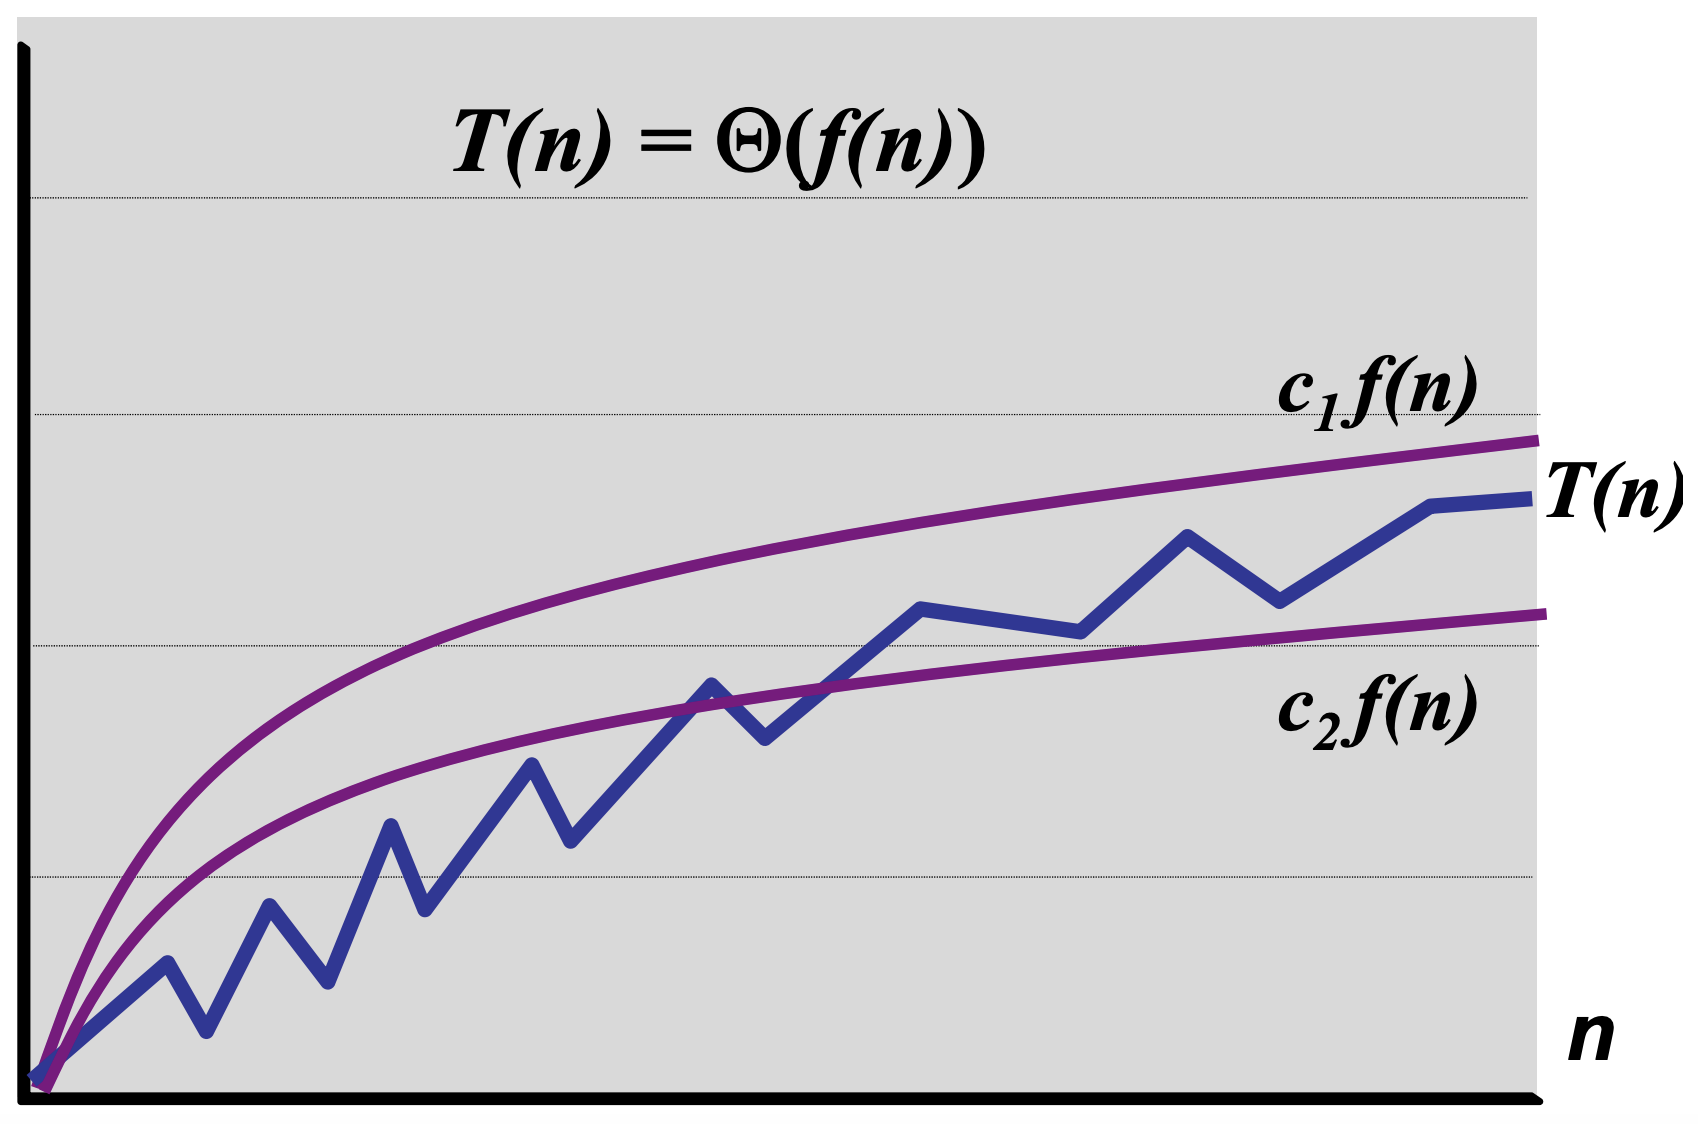
\includegraphics[width=0.55\linewidth]{cs2040s-big-theta.png}

    $T(n) = O(f(n))$ 
    \\* if $\exists c, n_0 > 0$ such that for all $n > n_0$, $T(n) \leq cf(n)$
    
    $T(n) = \Omega(f(n))$
    \\* if $\exists c, n_0 > 0$ such that for all $n > n_0$, $T(n) \geq cf(n)$
    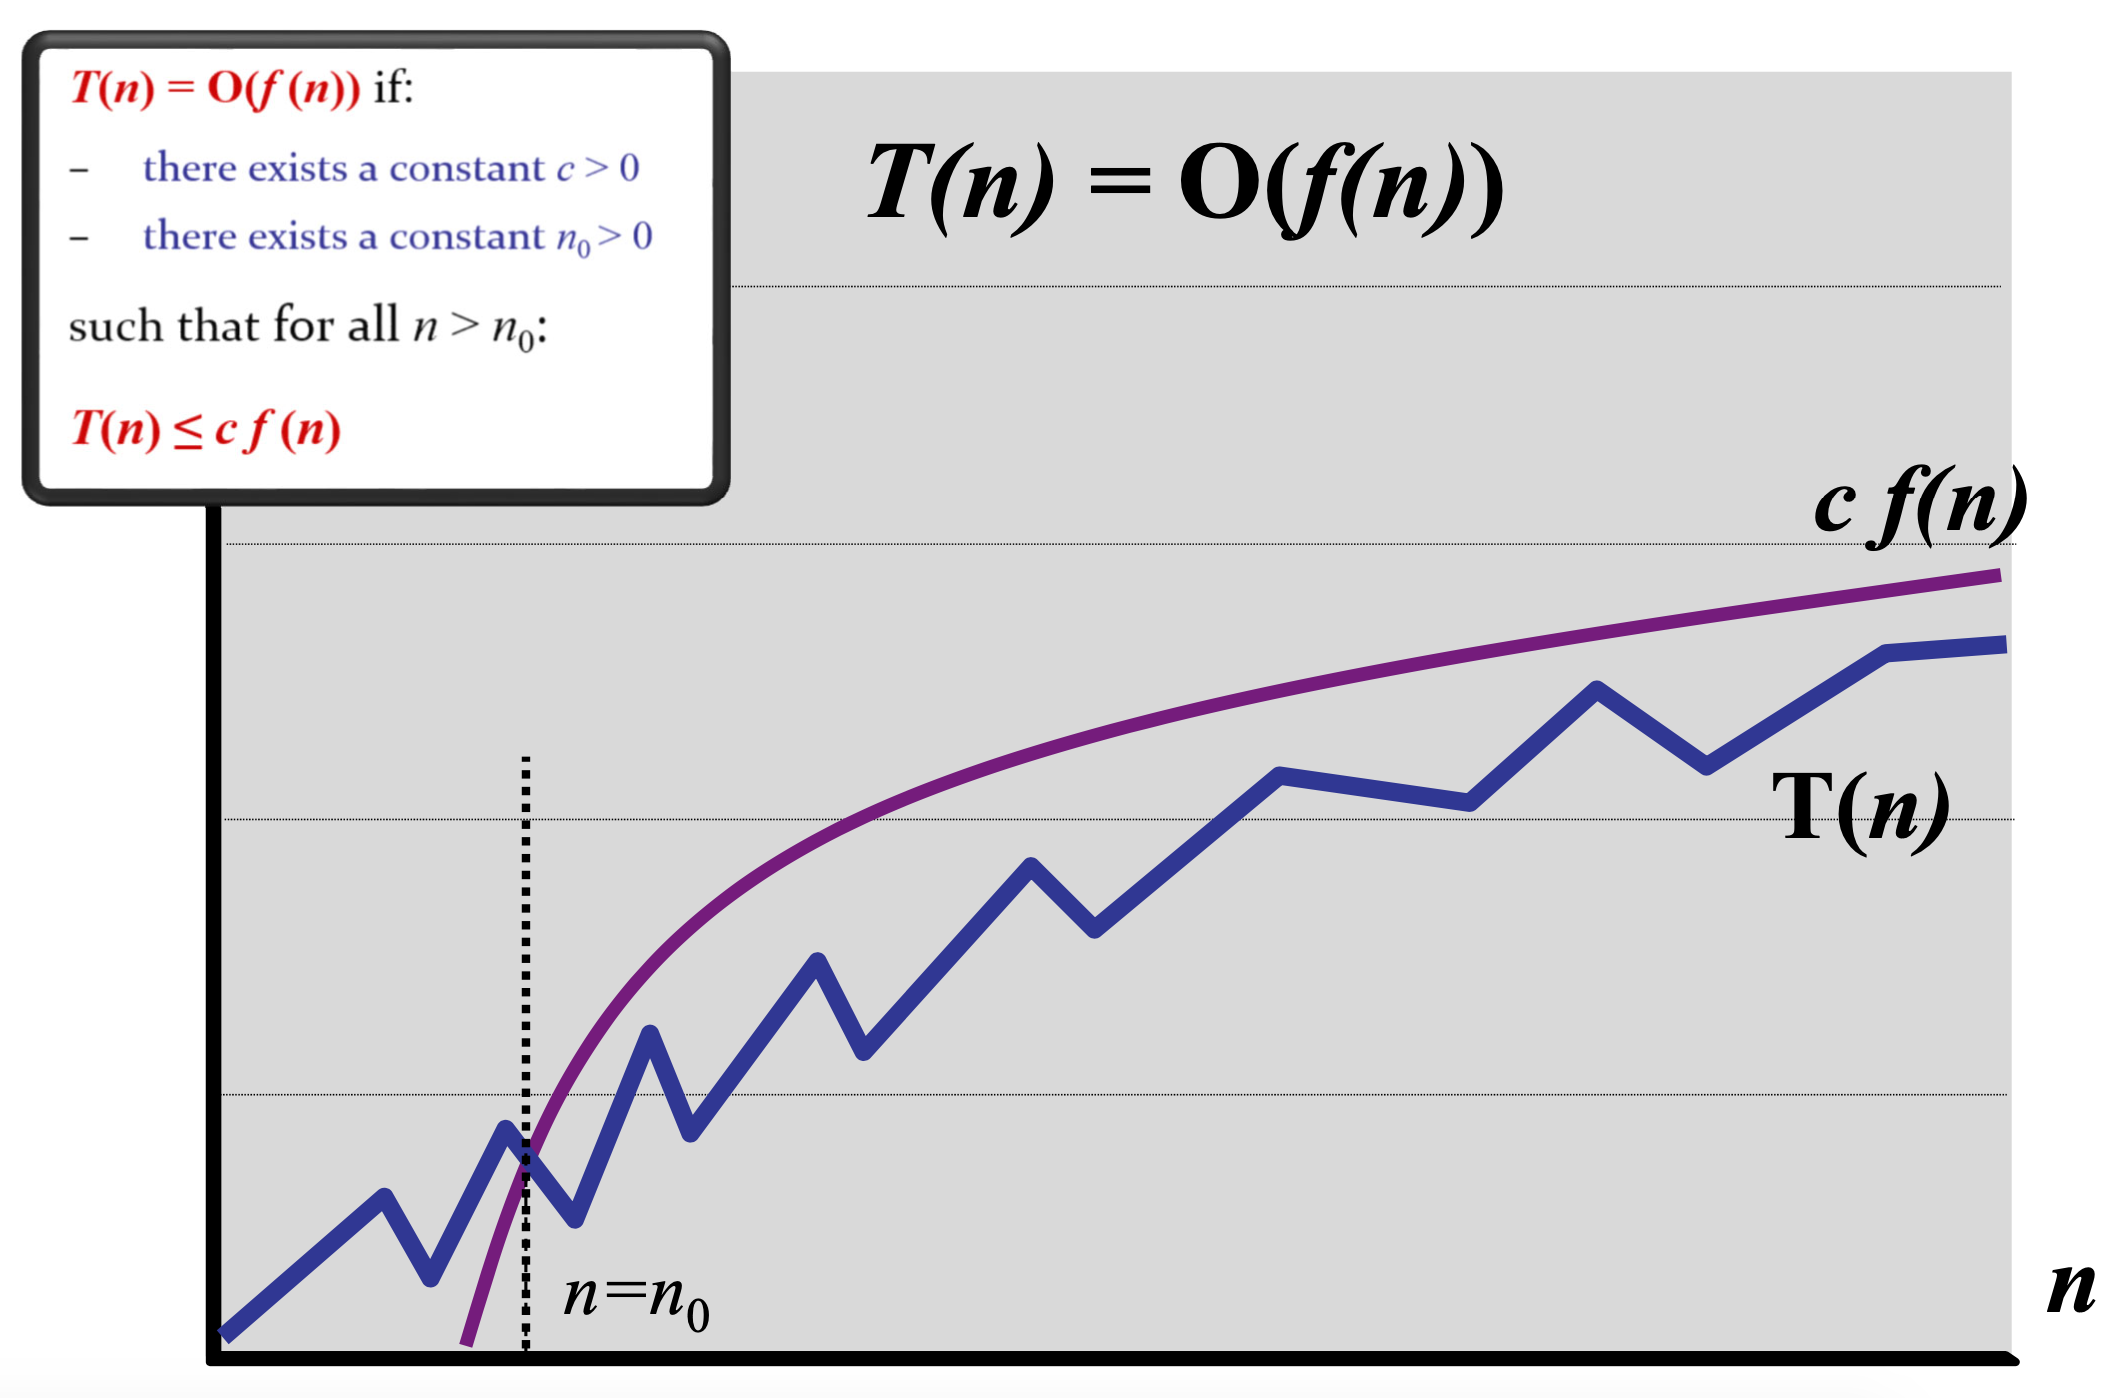
\includegraphics[width=0.48\linewidth]{cs2040s-big-o.png}
    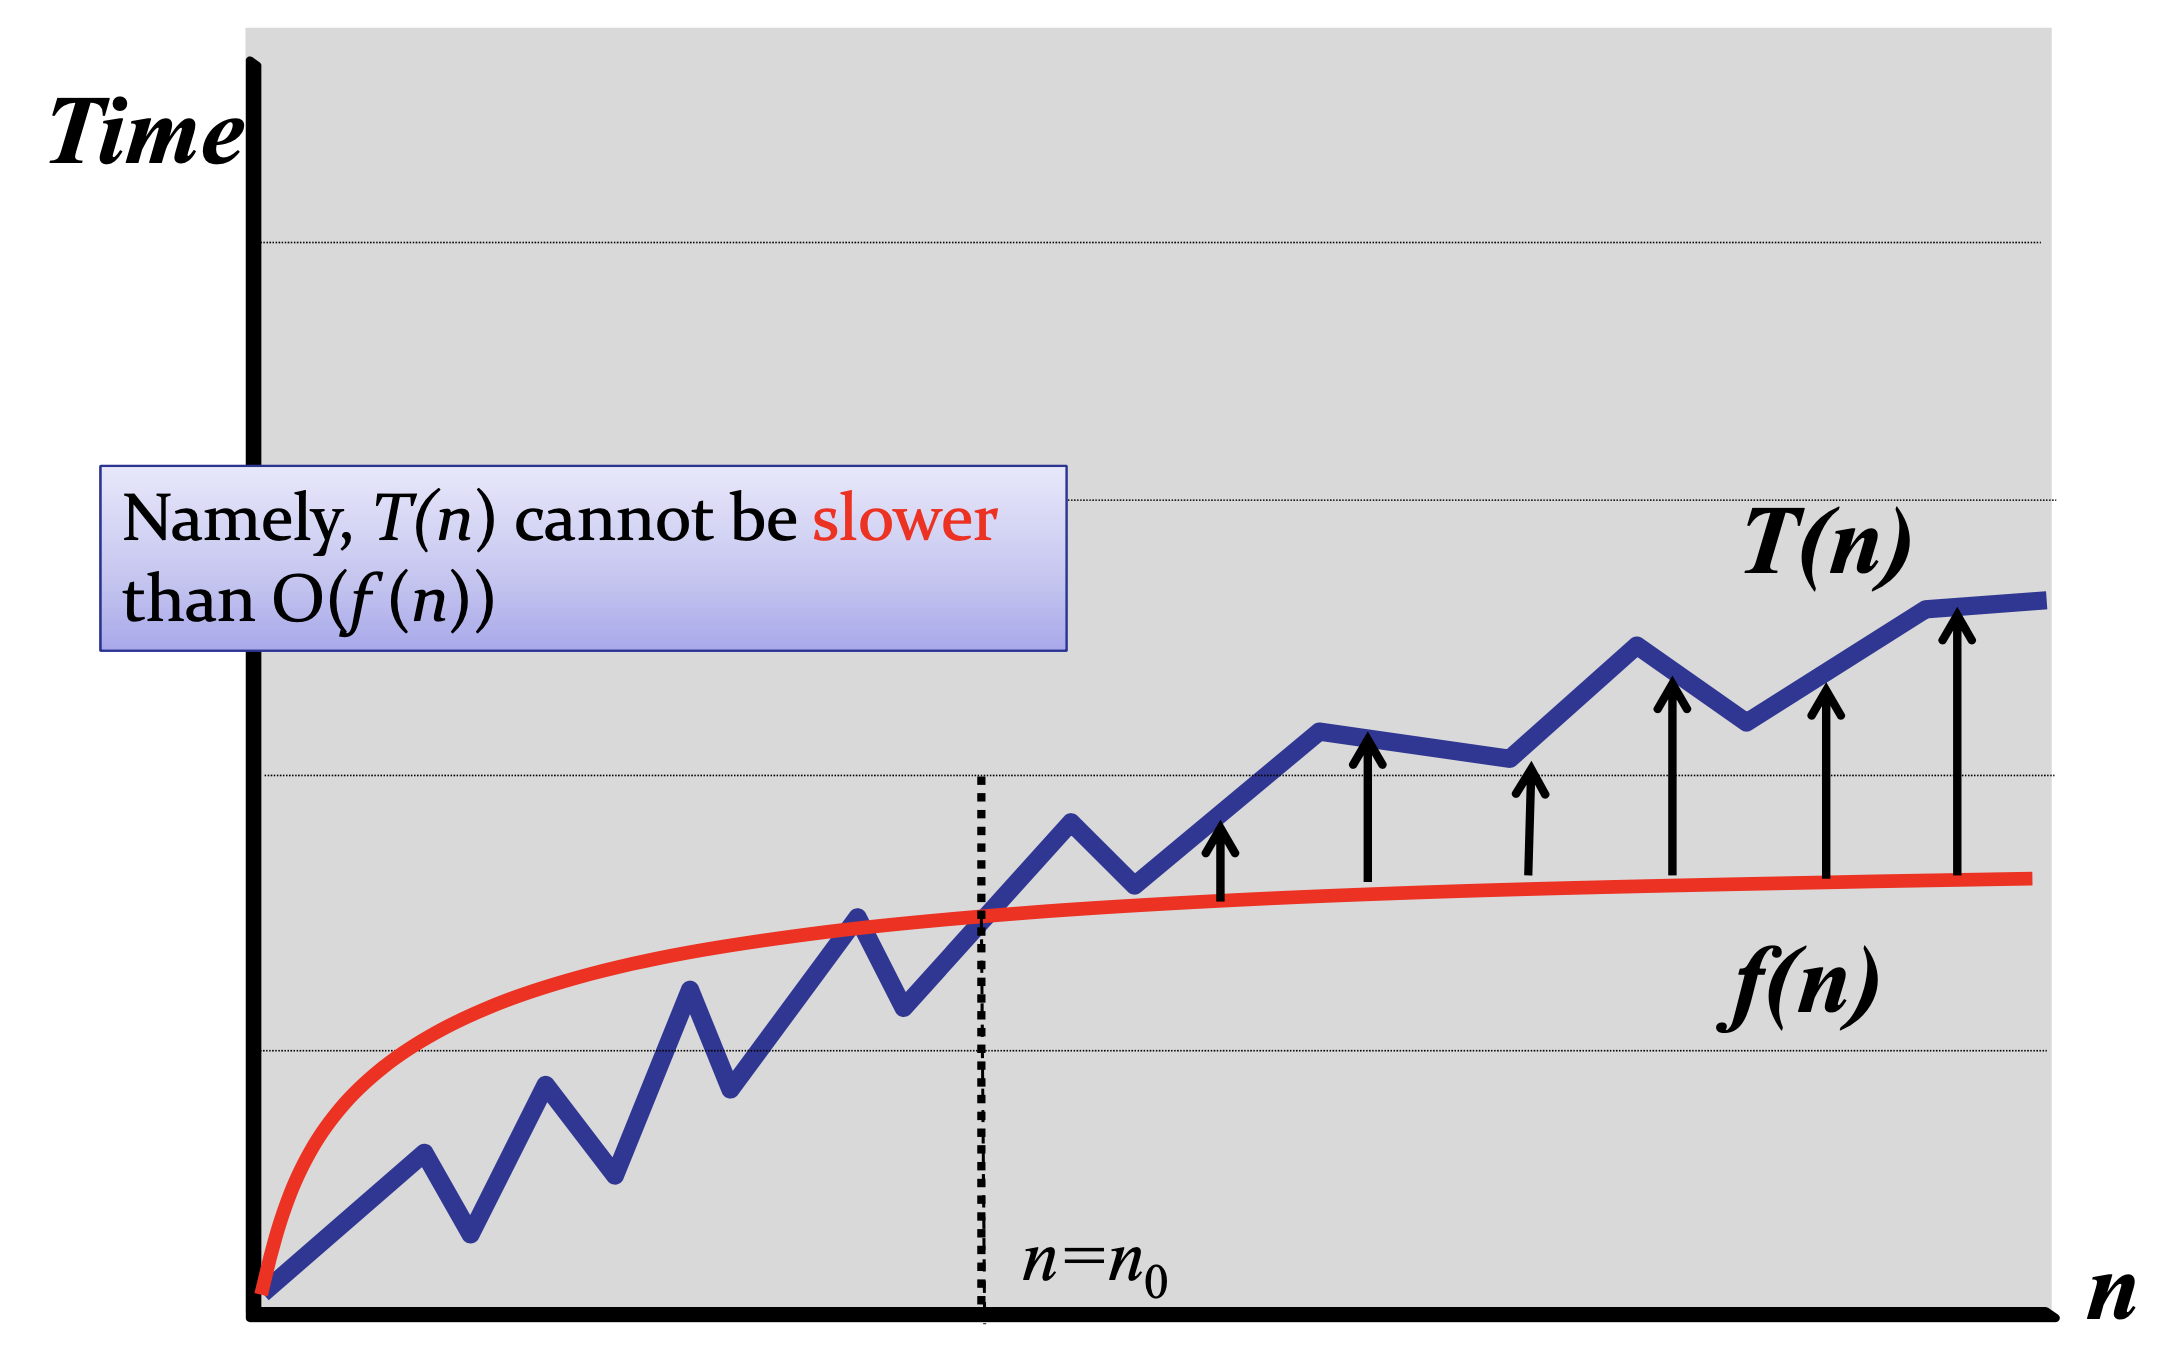
\includegraphics[width=0.48\linewidth]{cs2040s-big-omega.png}
    
\end{center}

\subsection{properties}
Let $T(n) = O(f(n))$ and $S(n) = O(g(n))$ 
\begin{itemize}
    \item addition: $T(n) + S(n) = O(f(n) + g(n))$
    \item multiplication: $T(n) * S(n) = O(f(n) * g(n))$
    \item composition: $f_1 \circ f_2 = O(g_1 \circ g_2)$
    \begin{itemize}
        \item only if both functions are increasing
    \end{itemize}
    \item if/else statements: $\text{cost} = \max(c1, c2) \leq c1+c2$
    \item max: $\max(f(n), g(n)) \leq f(n) + g(n)$
\end{itemize}

\subsubsection{notable}
\begin{itemize}
    \item $\sqrt{n}\log n$ is $O(n)$
    \item $O(2^{2n}) \neq O(2^n)$
    \item $O(\log (n!)) = O(n\log n) \then$ sterling's approximation
    \item $T(n-1) + T(n-2) + \dots + T(1) = 2T(n-1)$
\end{itemize}

\subsection{space complexity}
\begin{itemize}
    \item $\Theta(f(n))$ time complexity $\Then O(f(n))$ space complexity
    \item the maximum space incurred \textbf{at any time at any point} 
    \item NOT the maximum space incurred altogether!
    \item assumption: once we exit the function, we release all memory that was used
\end{itemize}

\section{SORTING}
\subsection{overview}
\begin{itemize}
    \item \textbf{BubbleSort} - compare adjacent items and swap 
    \item \textbf{SelectionSort} - takes the smallest element, swaps into place
    \item \textbf{InsertionSort} - from left to right: swap element leftwards until it's smaller than the next element. repeat for next element
    \begin{itemize}
        \item tends to be faster than the other $O(n^2)$ algorithms
    \end{itemize}
    \item \textbf{MergeSort} - mergeSort 1st half; mergeSort 2nd half; merge
    \item \textbf{QuickSort}
    \begin{itemize}
        \item partition algorithm: $O(n)$
        \item stable quicksort: $O(\log n)$ space
        \begin{itemize}
            \item first element as partition. 2 pointers from left to right
            \begin{itemize}
                \item left pointer moves until element > pivot
                \item right pointer moves until element < pivot
                \item swap elements until left = right. 
            \end{itemize}
            \item then swap partition and left=right index.
        \end{itemize}
    \end{itemize}
\end{itemize}

\subsection{optimisations of QuickSort}
\begin{itemize}
    \item array of duplicates: $O(n^2)$ without 3-way partitioning
    \item stable if the partitioning algo is stable.
    \item extra memory allows quickSort to be stable.
\end{itemize}

\subsubsection{choice of pivot}
\begin{itemize}
    \item worst case $O(n^2)$: first/last/middle element
    \item worst case $O(n\log n)$: median/random element
    \begin{itemize}
        \item split by fractions: $O(n\log n)$
    \end{itemize}
    \item choose at random: runtime is a random variable
\end{itemize}

\subsection{QuickSelect}
\begin{itemize}
    \item $O(n)$ - to find the $k^{\text{th}}$ smallest element
    \item after partitioning, the partition is always in the correct position
\end{itemize}

\section{TREES}
\subsection{binary search trees (BST)}
\begin{itemize}
    \item a BST is either empty, or a node pointing to 2 BSTs.
    \item tree balance depends on order of insertion
    \item balanced tree: $O(h) = O(\log n)$
    \item for a full-binary tree of size $n, \exists k \in \mathbb{Z}^+$ s.t. $n=2^k-1$ 
\end{itemize}

\subsubsection{BST operations}
\begin{itemize}
    \item \code{height, h(v) = max(h(v.left), h(v.right))}
    \begin{itemize}
        \item leaf nodes: \code{h(v)} = 0 
    \end{itemize}
    \item modifying operations
    \begin{itemize}
        \item \code{search}, \code{insert} - $O(h)$
        \item \code{delete} - $O(h)$
        \begin{itemize}
            \item case 1: no children - remove the node
            \item case 2: 1 child - remove the node, connect parent to child
            \item case 3: 2 children - delete the successor; replace node with successor
        \end{itemize}
    \end{itemize}
    \item query operations
    \begin{itemize}
        \item \code{searchMin} - $O(h)$ - recurse into left subtree
        \item \code{searchMax} - $O(h)$ - recurse into right subtree
        \item \code{successor} - $O(h)$
        \begin{itemize}
            \item if node has a right subtree: \code{searchMin(v.right)}
            \item else: traverse upwards and return the first parent that contains the key in its left subtree
        \end{itemize}
    \end{itemize}
\end{itemize}

\subsection{AVL Trees}
\begin{itemize}
    \item \textbf{height-balanced} (maintained with rotations)
    \begin{itemize}
        \item $\iff$ \code{|v.left.height - v.right.height| $\leq 1$}
    \end{itemize}
    \item each node is augmented with its height - \code{v.height = h(v)}
    \item space complexity: $O(LN)$ for $N$ strings of length $L$
\end{itemize}

\subsubsection{rebalancing}
[case 1] B is  \textbf{balanced: right-rotate}
\begin{center}
    $h(L) = h(M), \quad h(R) = h(M) - 1$
    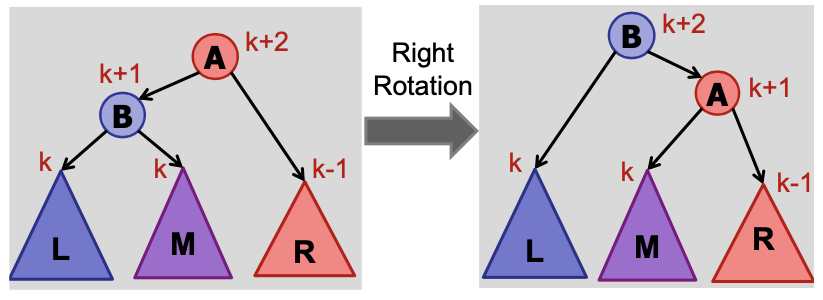
\includegraphics[width=0.65\linewidth]{cs2040s-rebalance-case-1.png}
\end{center}

[case 2] B is  \textbf{left-heavy: right-rotate}
\begin{center}
    $h(L) = h(M) + 1, \quad h(R) = h(M)$
    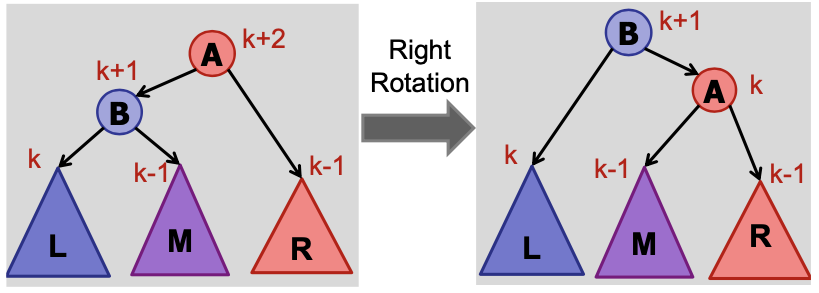
\includegraphics[width=0.65\linewidth]{cs2040s-rebalance-case-2.png}
\end{center}

[case 3] B is  \textbf{right-heavy: left-rotate(v.left), right-rotate(v)}
\begin{center}
    $h(L) = h(M) - 1, \quad h(R) = h(L)$
    \\* 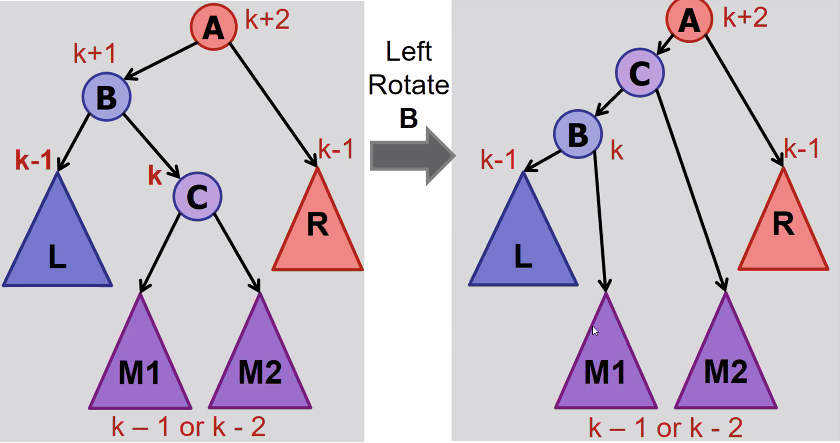
\includegraphics[width=0.65\linewidth]{cs2040s-rebalance-case-3-1.png}
    \\* 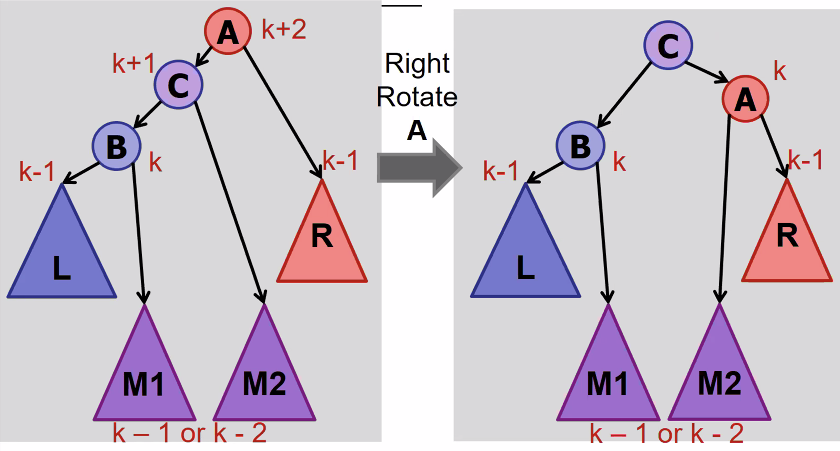
\includegraphics[width=0.65\linewidth]{cs2040s-rebalance-case-3-2.png}
\end{center}

\subsection{updating nodes after rotation}
\begin{center}
    weights
    \\* 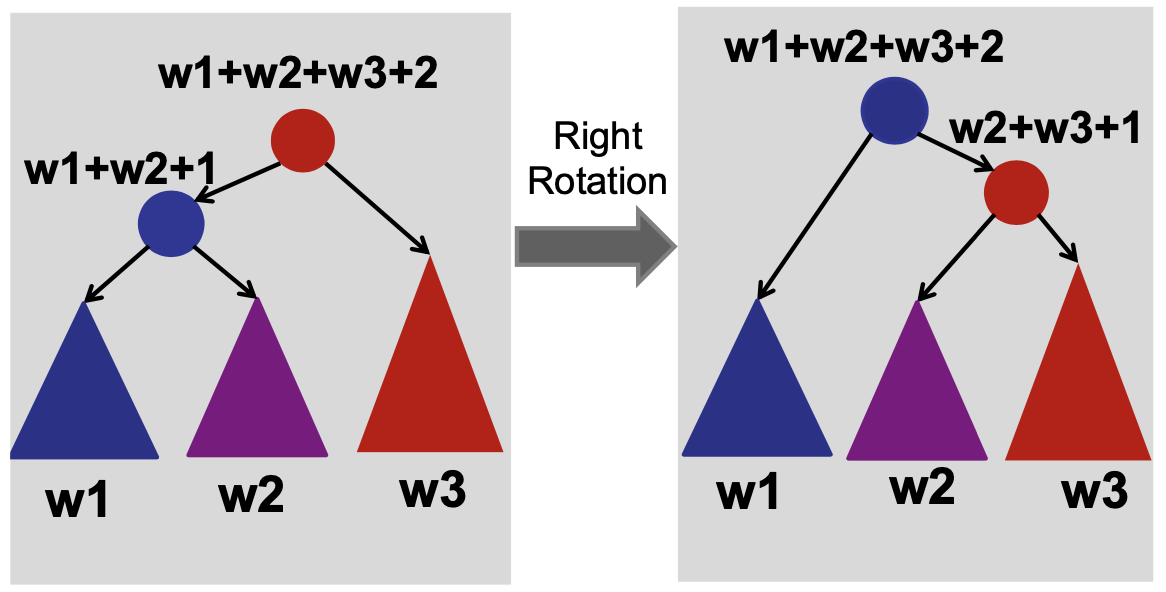
\includegraphics[width=0.65\linewidth]{cs2040s-rotate-weights.png}
    
    max
    \\* 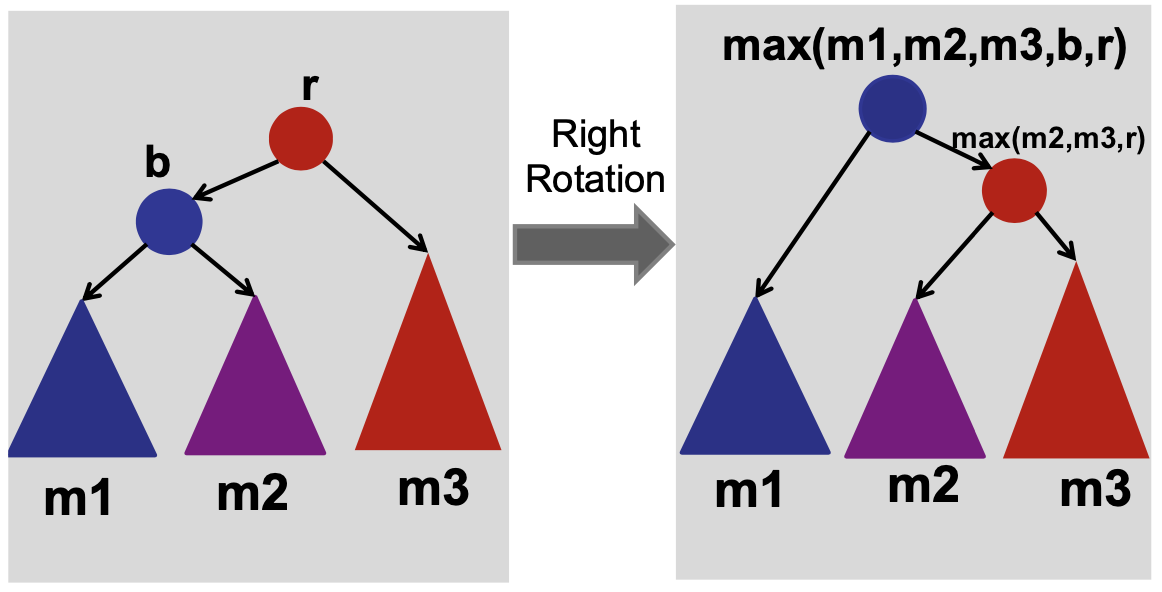
\includegraphics[width=0.65\linewidth]{cs2040s-rotate-max.png}
\end{center}

\begin{tightcenter}
    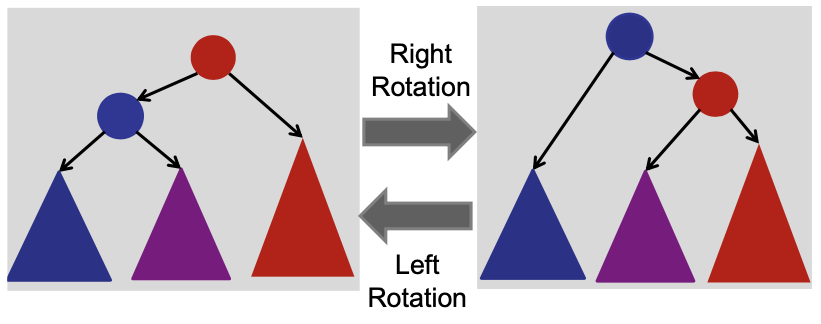
\includegraphics[width=0.8\linewidth]{cs2040s-tree-rotation.png}
\end{tightcenter}
\begin{itemize}
    \item insertion: max. 2 rotations
    \item deletion: recurse all the way up
    \item rotations can create every possible tree shape.
\end{itemize}

\subsection{Trie}
\begin{itemize}
    \item \code{search, insert} - $O(L)$ (for string of length $L$)
    \item space: $O($size of text $\cdot$ overhead$)$
\end{itemize}

\subsection{interval trees}
\begin{itemize}
    \item \code{search(key)} $\Then O(\log n)$
    \begin{itemize}
        \item if value is in root interval, return
        \item if value > max(left subtree), recurse right
        \item else recurse left (go left only when can't go right)
    \end{itemize}
    \item all-overlaps $\Then O(k \log n)$ for $k$ overlapping intervals
\end{itemize}

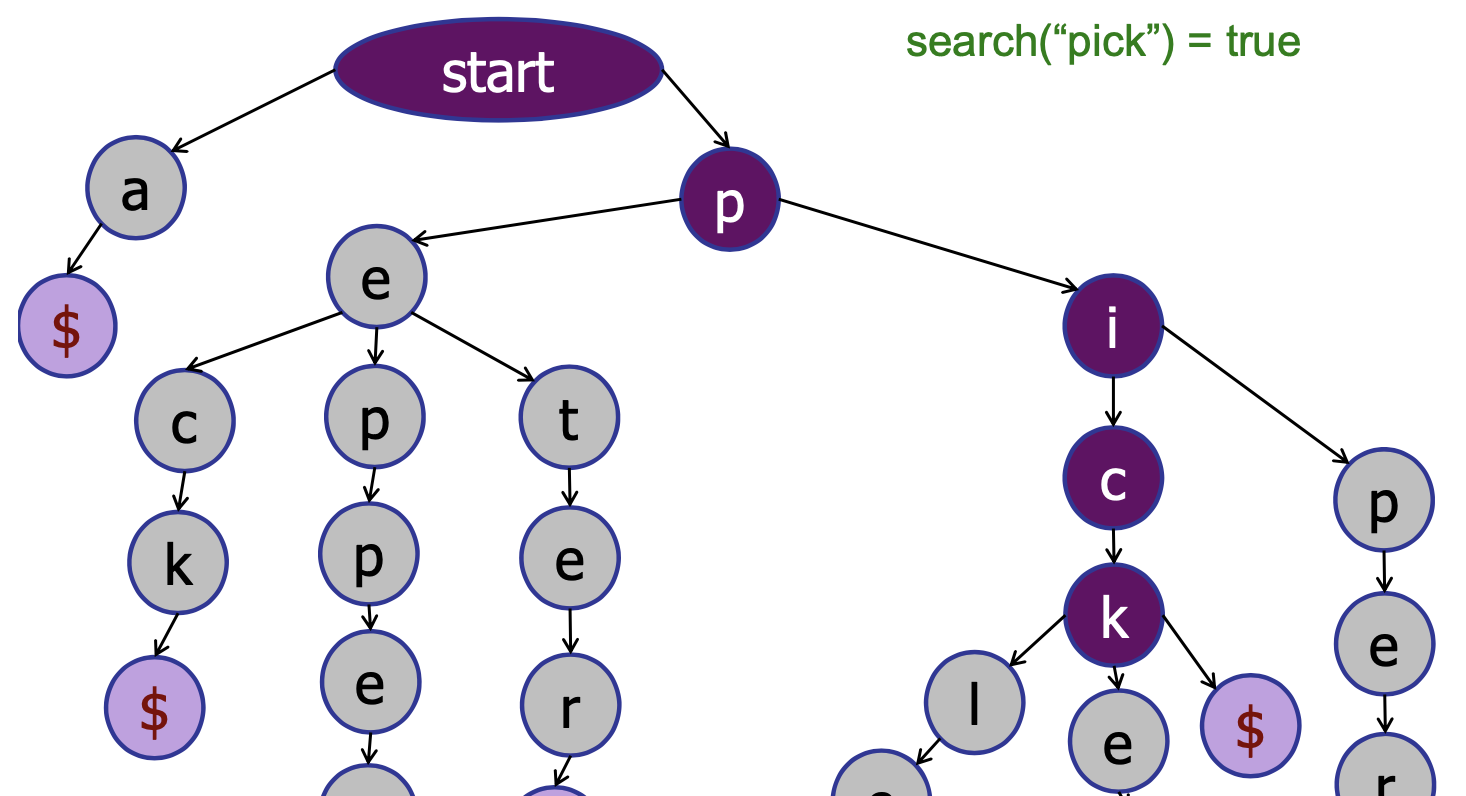
\includegraphics[width=0.5\linewidth]{cs2040s-trie.png}
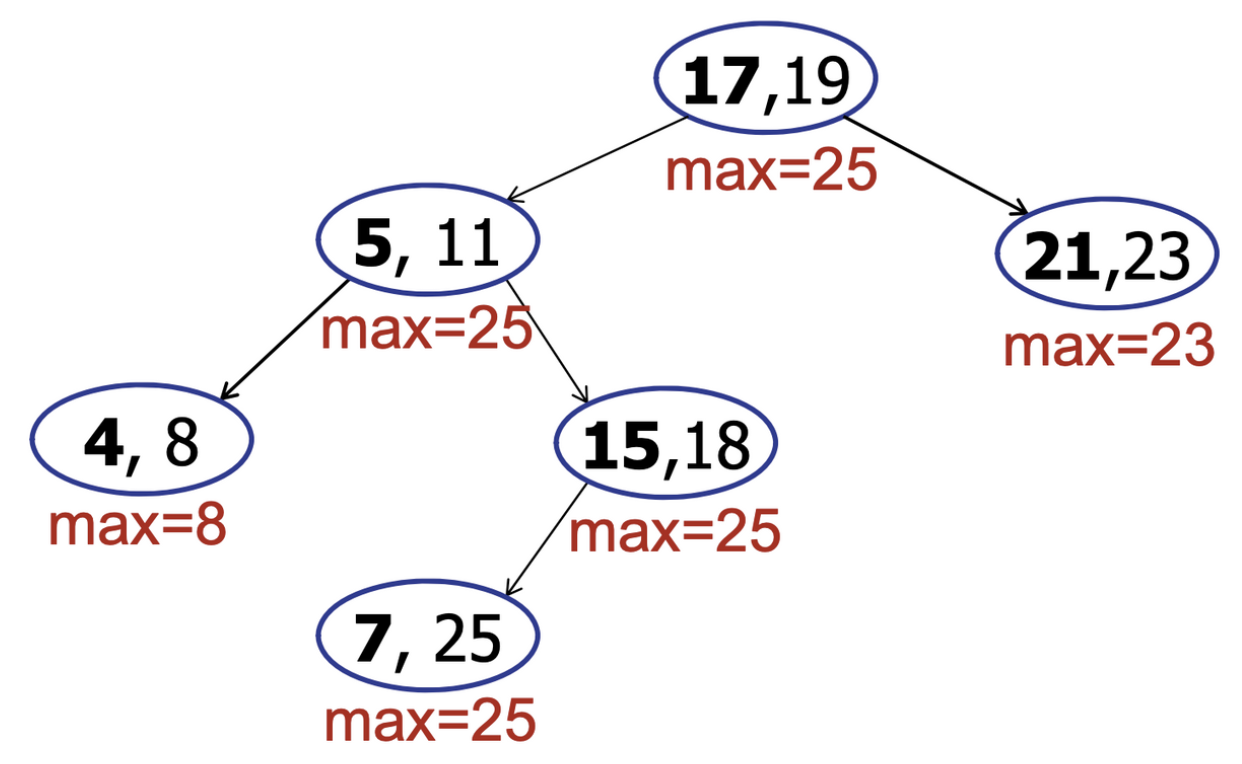
\includegraphics[width=0.45\linewidth]{cs2040s-interval-tree.png}

\subsection{orthogonal range searching}
\begin{itemize}
    \item binary tree; leaves store points, internal nodes store max value in left subtree
    \item \code{buildTree(points[])} $\Then O(n \log n)$ \quad (space is $O(n)$)
    \item \code{query(low, hight)} $\Then O(k + \log n)$ for $k$ points
    \begin{itemize}
        \item \code{v=findSplit()} $\Then O(\log n)$ - find node b/w low \& high
        \item \code{leftTraversal(v)} $\Then O(k)$ - either output all the right subtree and recurse left, or recurse right 
        \item \code{rightTraversal(v)} - symmetric
    \end{itemize}
    \item \code{insert(key), insert(key)} $\Then O(\log n)$ 
    \item \code{2D\_query()} $\Then O(\log^2n + k)$ \quad (space is $O(n \log n)$)
    \begin{itemize}
        \item build x-tree from x-coordinates; for each node, build a y-tree from y-coordinates of subtree
    \end{itemize}
    \item \code{2D\_buildTree(points[])} $\Then O(n \log n)$
\end{itemize}

\subsection{kd-Tree}
\begin{tightcenter}
    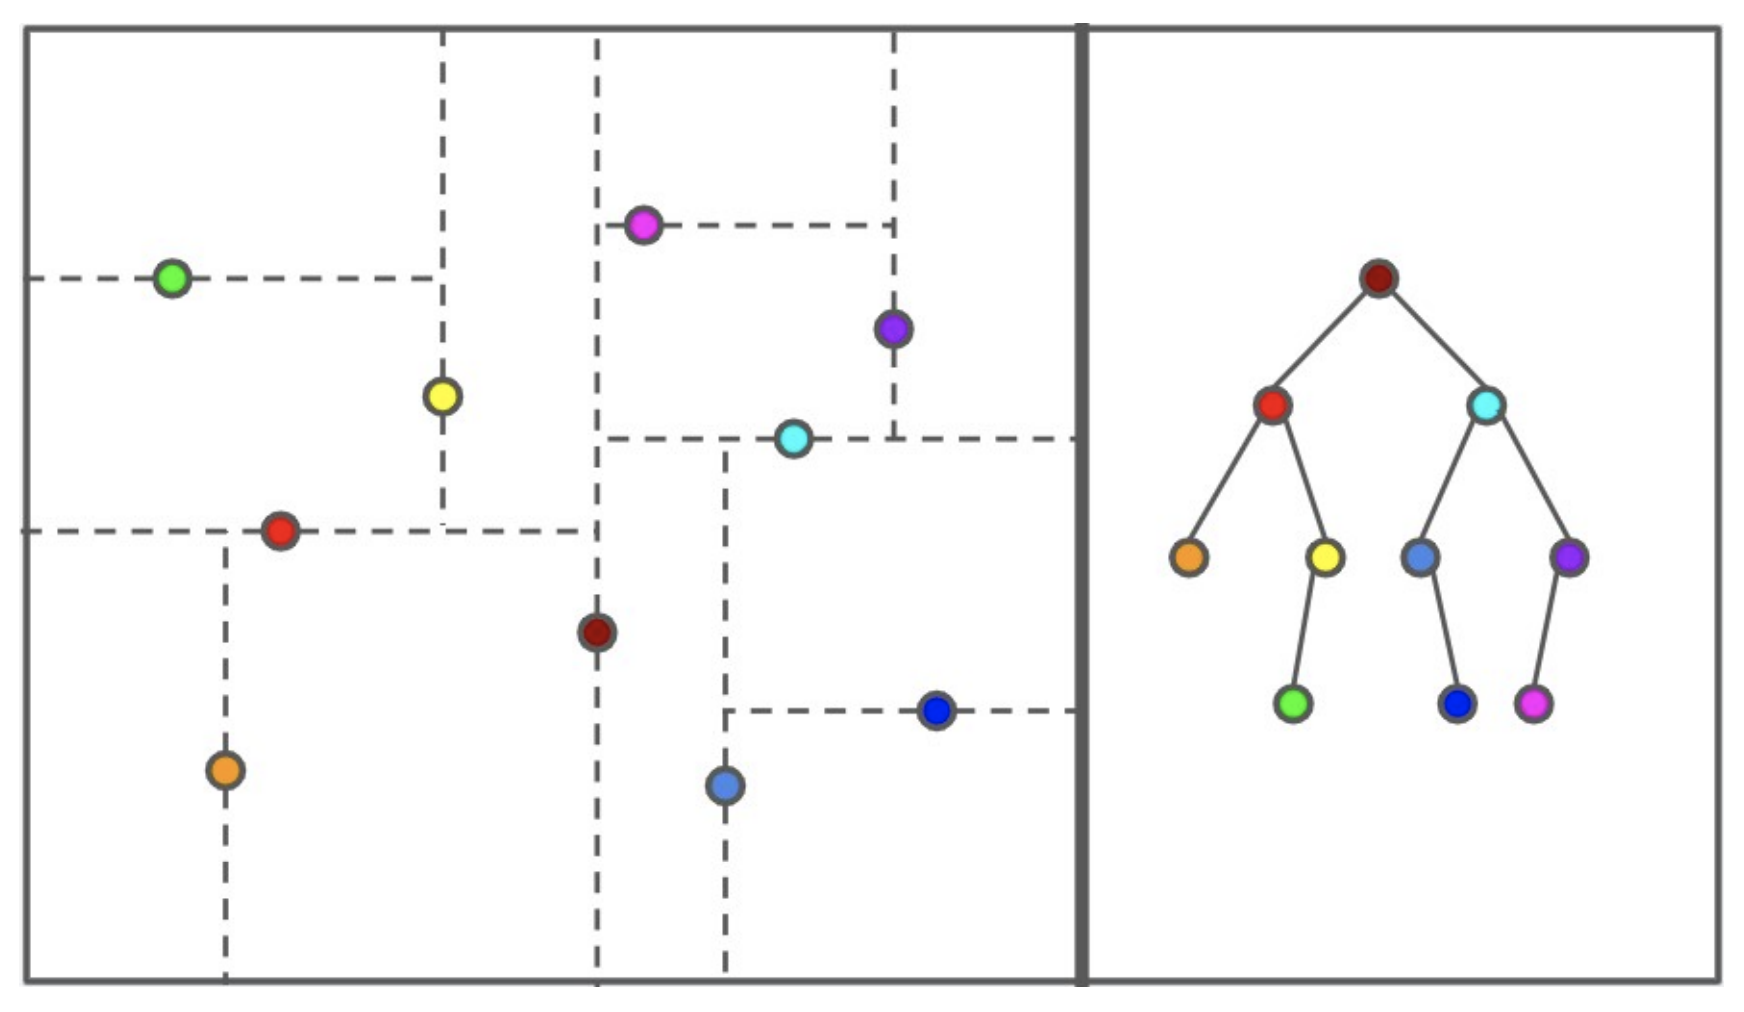
\includegraphics[width=0.6\linewidth]{cs2040s-kdtree.png}
\end{tightcenter}
\begin{itemize}
    \item stores geometric data (points in an $(x, y)$ plane)
    \item alternates splitting (partitioning) via $x$ and $y$ coordinates
    \item \code{construct(points[])} $\Then O(n \log n)$
    \item \code{search(point)} $\Then O(h)$
    \item \code{searchMin()} $\Then T(n) = 2T(\frac{n}{4}) + O(1) \Then O(\sqrt{n})$
\end{itemize}

\subsection{(a, b)-trees}
{\scriptsize{e.g. a (2, 4)-tree storing 18 keys}}
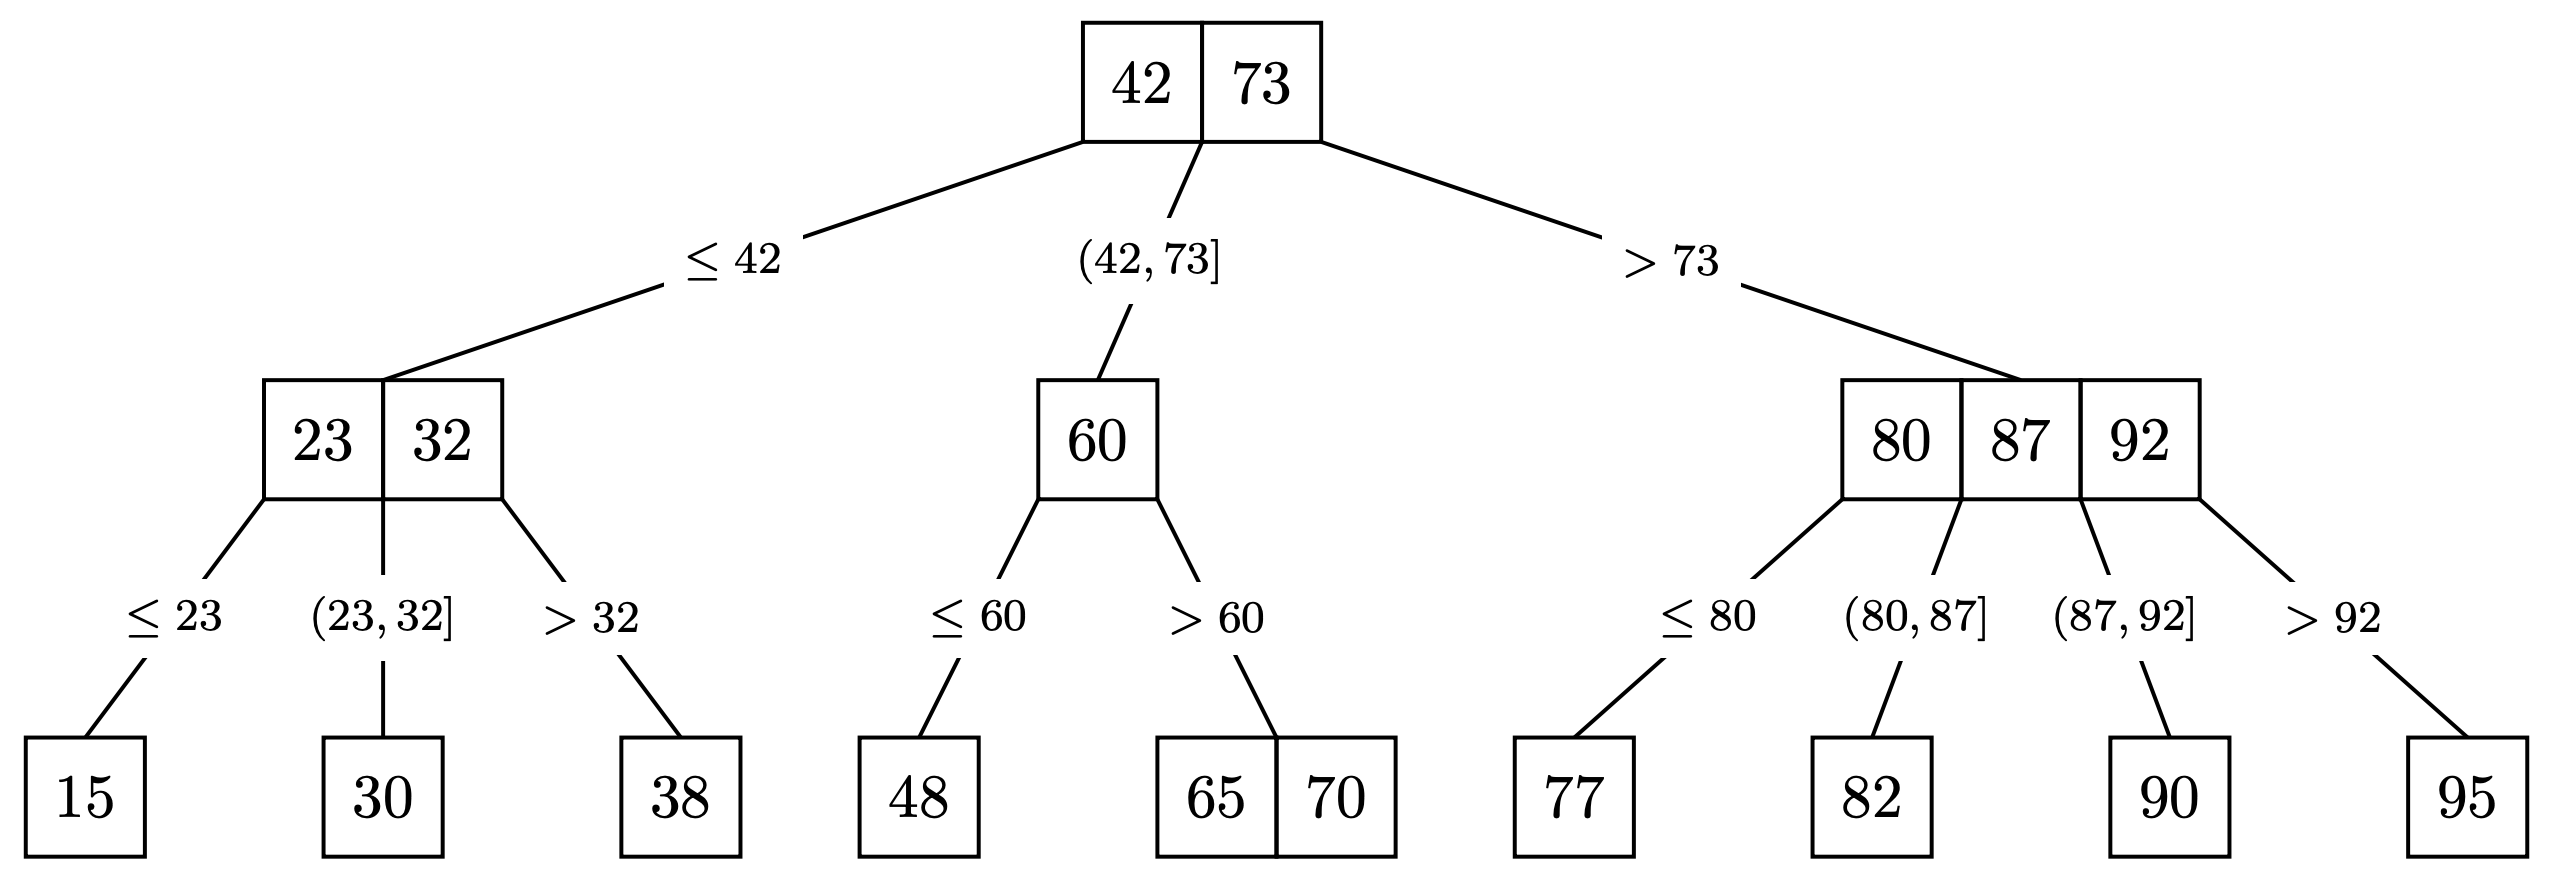
\includegraphics[width=1\linewidth]{cs2040s-ab-tree.png}
\begin{itemize}
    \item rules
    \begin{enumerate}
        \item $(a, b)$-child policy where $2 \leq a \leq (b+1)/2$
        \begin{tabular}{|c|c|c|c|c|}
            \hline 
             & \multicolumn{2}{c|}{\# keys} & \multicolumn{2}{c|}{\# children}
            \\\hline
            node type & min & max & min & max
            \\\hline
            root & $1$ & $b-1$ & $2$ & $b$
            \\\hline
            internal & $a-1$ & $b-1$ & $a$ & $b$
            \\\hline
            leaf & $a-1$ & $b-1$ & $0$ & $0$
            \\\hline
        \end{tabular}
        \item an internal node has 1 more child than its number of keys
        \item all leaf nodes must be at the \textbf{same depth} from the root
    \end{enumerate}
    \item terminology (for a node $z$)
    \begin{itemize}
        \item key range - range of keys covered in subtree rooted at $z$
        \item keylist - list of keys within $z$
        \item treelist - list of $z$'s children
    \end{itemize}
    \item max height $= O(\log_an) + 1$
    \item min height $= O(\log_bn)$
    \item \code{search(key)} $\Then O(\log n)$
    \begin{itemize}
        \item $= O(\log_2 b \cdot \log_a n)$ for binary search at each node
    \end{itemize}
    \item \code{insert(key)} $\Then O(\log n)$
    \item \code{split()} a node with too many children
    \begin{enumerate}
        \item use median to split the keylist into 2 halves
        \item move median key to parent; re-connect remaining nodes
        \item (if the parent is now unbalanced, recurse upwards; if the root is reached, median key becomes the new root)
    \end{enumerate}
    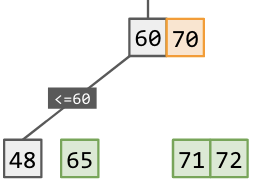
\includegraphics[width=0.4\linewidth]{cs2040s-abtree-split-1.png}
    $\Then$
    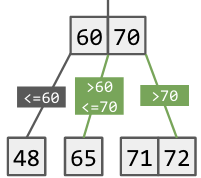
\includegraphics[width=0.3\linewidth]{cs2040s-abtree-split-2.png}
    \item \code{delete(key)} $\Then O(\log n)$
    \begin{itemize}
        \item if the node becomes empty, \code{merge(y, z)} - join it with its left sibling \& replace it with their parent
        \\* 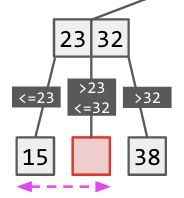
\includegraphics[width=0.25\linewidth]{cs2040s-abtree-delete-1.png}
        $\Then$
        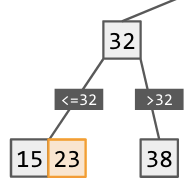
\includegraphics[width=0.3\linewidth]{cs2040s-abtree-delete-2.png}
        \item if the combined nodes exceed max size: \code{share(y, z)} = \code{merge(y, z)} then \code{split()}
    \end{itemize}
\end{itemize}

\subsection{B-Tree}
\begin{itemize}
    \item $(B, 2B)$-trees $\Then (a, b)$-tree where $a=B, b=2B$ 
    \item possible augmentation: use a linkedList to connect between each level
\end{itemize}

\end{multicols}

\hrulefill \\

\begin{multicols}{2}
    % what is going on with the headers here?
    % whatttaaatt

    \begin{tightcenter}
        $
        \begin{array}{| c | c | c | c | c | c |}
            \hline\textbf{sort} & \textbf{best} & \textbf{average} & \textbf{worst} & \textbf{stable?} & \textbf{memory}
    
            \\\hline\text{bubble} & \Omega(n) & O(n^2) & O(n^2) & \checkmark & O(1)
            
            \\\hline\text{selection} & \Omega(n^2) & O(n^2) & O(n^2) & \times & O(1)
            
            \\\hline\text{insertion} & \Omega(n) & O(n^2) & O(n^2) & \checkmark & O(1)
            
            \\\hline\text{merge} & \Omega(n\log n) & O(n\log n) & O(n\log n) & \checkmark & O(n)
            
            \\\hline\text{quick} & \Omega(n\log n) & O(n\log n) & O(n^2) & \times & O(1)
            \\\hline
        \end{array} 
        $\
        \begin{tabular}{| c | c |}
            \multicolumn{2}{c}{Sorting Invariants}
            \\\hline\textbf{sort} & \textbf{invariant} (after $k$ iterations)
            \\\hline bubble & largest $k$ elements are sorted
            \\\hline selection & smallest $k$ elements are sorted
            \\\hline insertion & first $k$ slots are sorted
            \\\hline merge & given subarray is sorted
            \\\hline quick & partition is in the right position
            \\\hline
        \end{tabular} \begin{tabular}{| c | c |}
            \multicolumn{2}{c}{Searching}\\\hline
            \textbf{search} & \textbf{average} \\\hline
            linear & $O(n)$ \\\hline
            binary & $O(\log n)$ \\\hline
            quickSelect & $O(n)$ \\\hline
            interval & $O(\log n)$ \\\hline
            all-overlaps & $O(k\log n)$ \\\hline
            1D range & $O(k + \log n)$ \\\hline
            2D range & $O(k + \log^2 n)$ \\\hline
        \end{tabular}

        \vspace{5pt}
        Data Structures Assuming $O(1)$ Comparison Cost
        \\* \begin{tabular}{| c | c | c |}\hline
            \textbf{data structure} & \textbf{search} & \textbf{insert}\\\hline
            sorted array & $O(\log n)$ & $O(n)$ \\\hline
            unsorted array & $O(n)$ & $O(1)$ \\\hline
            linked list & $O(n)$ & $O(1)$ \\\hline
            tree (kd/(a, b)/binary) & $O(\log n)$ or $O(h)$ & $O(\log n)$ or $O(h)$ \\\hline
            trie & $O(L)$ & $O(L)$ \\\hline
            dictionary & $O(\log n)$ & $O(\log n)$ \\\hline
            symbol table & $O(1)$ & $O(1)$ \\\hline
            chaining & $O(n)$ & $O(1)$ \\\hline
            open addressing & $\frac{1}{1-\alpha} = O(1)$ & $O(1)$ \\\hline
        \end{tabular}

        \ 
        \subsection{Orders of Growth}
        \begin{gather*}
            1 < \log n < \sqrt{n} < n < n \log n < n^2 < n^3 < 2^n < 2^{2n} \\
            \log_a n < n^a < a^n < n! < n^n
        \end{gather*}
        Note that:
        \begin{equation*}
            3^n \neq O(2^n) \text{ and } 2^{log(n)} = O(n)
        \end{equation*}
        \begin{align*}
            T(n) &= 2T(\frac{n}{2}) + O(n) &\Rightarrow O(n \log n)
            \\ T(n) &= T(\frac{n}{2}) + O(n) &\Rightarrow O(n)
            \\ T(n) &= 2T(\frac{n}{2}) + O(1) &\Rightarrow O(n)
            \\ T(n) &= T(\frac{n}{2}) + O(1) &\Rightarrow O(\log n)
            \\ T(n) &= 2T(n - 1) + O(1) &\Rightarrow O(2^n)
            \\ T(n) &= 2T(\frac{n}{2}) + O(n \log n) &\Rightarrow O(n(\log n)^2)
            \\ T(n) &= 2T(\frac{n}{4}) + O(1) &\Rightarrow O(\sqrt{n})
            \\ T(n) &= T(n - c) + O(n) &\Rightarrow O(n^2)
        \end{align*}
    \end{tightcenter}
\end{multicols}
\end{document}